\documentclass[a4paper]{article}

\usepackage[swedish]{babel}
\usepackage[utf8]{inputenc}
\usepackage[T1]{fontenc}
\usepackage{amsmath}
\usepackage{amssymb}
\usepackage[T1]{fontenc}
\usepackage{graphicx}
\usepackage{epstopdf}
\usepackage{placeins}

\begin{document}

\section*{2.1}

Resultatet för alla deluppgifter jämfördes med Maple (se appendix \ref{ap:maple}). För det mesta stämde resultatet överens med det som beräknades för hand. Däremot så sa Maple att g) konvergerar, vilket den inte gör enligt handräkning. Därutöver kände inte Maple igen serierna i e) och f).

\subsection*{a)}
För att se om serien $\sum_{k=2}^{+\infty}\frac{3}{k^2-k}$ konvergergerar
används jämförelsetestet på gränsvärdesform med den kända (konvergenta) p-serien
$\sum_{k=2}^{+\infty}\frac{1}{k^2}$

\begin{align*}
  \lim_{k\to\infty} \frac{\frac{3}{k^2-k}}{\frac{1}{k^2}} = \lim_{k\to\infty}
  \frac{3}{1 - \frac{1}{k}} = 3,
\end{align*}

\noindent eftersom gränsvärdet existerar och p-serien är konvergent, så måste den andra serien även också vara det.

\subsection*{b)}

För att se om $\sum_{k=1}^{+\infty}\frac{k}{(k+i)^3}$ så kollar vi om serien är
absolutkonvergent för att bli av med $i$:et

\begin{align*}
  \left|\frac{k}{(k+i)^3}\right| = \frac{k}{\left| k+i \right|^2\cdot\left| k + i \right|} = \frac{k}{(k^2+1)\sqrt{k^2+1}} < \frac{k}{k^2+1},
\end{align*}

\noindent en jämförelse görs nu med $\frac{k}{k^2+1}$ som konvergerar enligt
jämförelsetestet med den konvergenta p-serien med $p=2$

\begin{align*}
  \lim_{k\to\infty} \frac{\frac{k}{k^2+1}}{\frac{1}{k^2}} = \lim_{k\to\infty} \frac{k^3}{k^2+1} = \lim_{k\to\infty} \frac{1}{1/k^2 + 1/k} = 0.
\end{align*}

\noindent Alltså är $\frac{k}{k^2+1}$ konvergent enligt jämförelsetestet på
gränsvärdesform, vilket medför att $\sum_{k=1}^{+\infty}\frac{k}{(k+i)^3}$ är
absolutkonvergent och därmed även konvergent enligt jämförelsetestet.

\subsection*{c)}

Serien $\sum_{k=1}^{+\infty}\frac{(-1)^k}{\sqrt{k}}$ är alternerande och
uppfyller Leibniz test, d.v.s.

\begin{align*}
  \left| \frac{(-1)^k}{\sqrt{k}} \right| = \frac{1}{\sqrt{k}} \to 0, k \to \infty,
\end{align*}

\noindent är avtagande och har gränsvärdet $0$ då $k\to\infty$. Serien är därmed
konvergent enligt Leibniz test.

\subsection*{d)}

För att se om $\sum_{k=1}^{+\infty}\frac{k^3}{3^k}$ är konvergent så används
kvottestet

\begin{align*}
 \kappa &= \lim_{k\to\infty} \frac{\left| \frac{(k+1)^3}{3^{k+1}} \right|}{\left| \frac{k^3}{3^k} \right|}
          = \lim_{k\to\infty} \frac{3^k}{3^{k+1}}\cdot\frac{(k+1)^3}{k^3}\\
  &= \lim_{k\to\infty} \frac{1}{3}\left( 1 + \frac{k^2}{k^3} + \frac{k}{k^3} + \frac{1}{k^3} \right) = \frac{1}{3},
\end{align*}

\noindent eftersom $\kappa$ existerar och är mindre än $1$ så är serien
$\sum_{k=1}^{+\infty}\frac{k^3}{3^k}$ absolutkonvergent och därmed även konvergent.

\subsection*{e)}

Är $\sum_{k=0}^{+\infty}e^{-ik}$ konvergent?

Eftersom den ovanstående summan kan skrivas som en geometrisk serie
$\sum_{k=0}^{+\infty}Cr^k$, där $k = 1$, $r = e^{-i}$ och $|r| = 1$, så måste
ursprungsserien vara divergent eftersom den kan skrivas som en divergent
geometrisk serie.

\subsection*{f)}

Är $\sum_{k=1}^{+\infty}\frac{1}{k^{1+1/k}}$ konvergent?

Jämförelsetestet med den divergenta harmoniska serien $\frac{1}{k}$ ger

\begin{align*}
  L = \lim_{k\to\infty} \frac{\frac{1}{k^{1+1/k}}}{\frac{1}{k}} &= \lim_{k\to\infty}k^{1-(1+1/k)} = \lim_{k\to\infty}k^{-1/k} = \lim_{k\to\infty}\frac{1}{k^{1/k}}\\ &= \lim_{k\to\infty} \frac{1}{e^{\ln(k^{1/k})}} = \lim_{k\to\infty} \frac{1}{e^{\frac{\ln k}{k}}} = 1,
\end{align*}

\noindent eftersom $\frac{\ln k}{k} \to 0, k \to \infty$. Då gränsvärden $L = 1$ existerar och $\frac{1}{k}$ ger en divergent harmonisk serie, så måste även
ursprungsserien vara divergent.

\subsection*{g)}

För att avgöra om $\sum_{k=1}^{+\infty}\frac{(-1)^k}{\arctan k}$ är konvergent
eller divergent undersöks seriens termer. Eftersom

\begin{align*}
  \left| \frac{(-1)^k}{\arctan k} \right| = \frac{1}{\arctan k} \to \frac{2}{\pi}, k \to \infty,
\end{align*}

\noindent så måste serien vara divergent då termerna inte går mot noll. Notera att den
första likheten käller då $k > 0$.

\subsection*{h)}

För att se om

\begin{align*}
  \sum_{k=1}^{+\infty} \frac{(-1)^k\sin k}{k^2 + 1}
\end{align*}

\noindent är konvergent eller inte så undersöks serien för absolutkonvergens och eftersom 

\begin{align*}
  \left| \frac{(-1)^k\sin k}{k^2 + 1} \right| \leq \frac{1}{k^2 + 1} < \frac{1}{k^2},
\end{align*}

\noindent är $\frac{1}{k^2}$ är en känd konvergerande p-serie, vilket medför att
ursprungsserien måste vara absolutkonvergent och därmed konvergent.

\section*{2.2}

Här användes \textsc{Matlab} för att illustrera delsummorna till

\begin{align}
  \frac{3\pi}{4} + \sum_{k=1}^{+\infty}\frac{(-1)^k-1}{\pi k^2}\cos (kt) + \frac{1}{k}\sin (kt).\label{eq:22fourier}
\end{align}

\noindent se Figur \ref{fig:serie22}

\begin{figure}[h!]
  \centering
  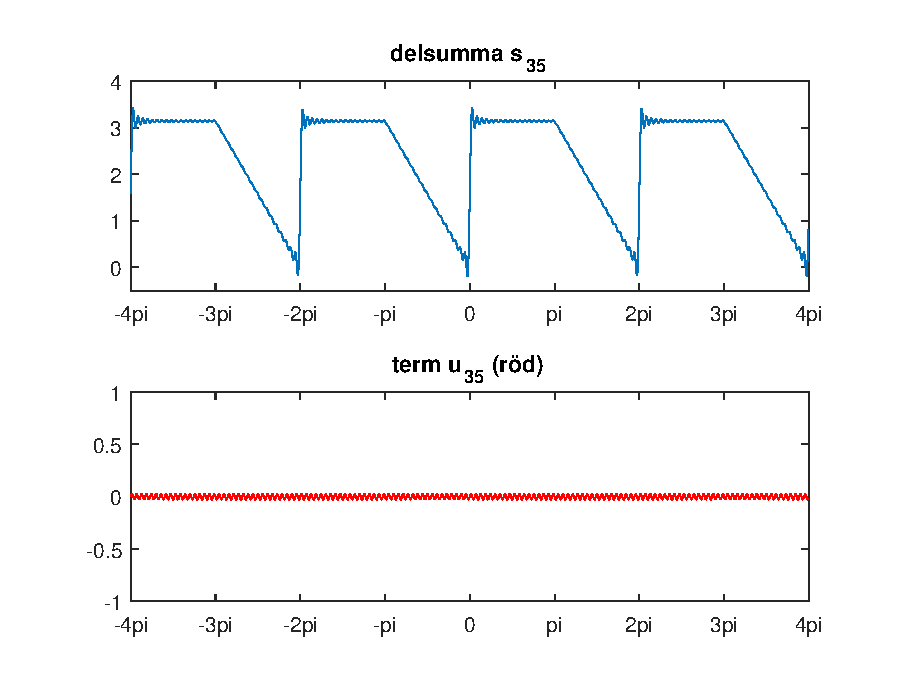
\includegraphics[width=0.75\linewidth]{serie22.eps}
  \caption{}
  \label{fig:serie22}
\end{figure} 

\noindent Härefter gjordes gissningen att (\ref{eq:22fourier}) utvecklas till funktionen

\begin{align*}
  f(t) =
  \begin{cases}
    \pi, 0 \leq t < \pi,\\
    -t + 2\pi, \pi \leq t \leq 2\pi
  \end{cases}.
\end{align*}

För att bekräfta detta tas Fourierkoefficienterna fram ur definitionen av
den trigonometriska Fourierserien för $f(t)$, d.v.s.

\begin{align*}
  \mathcal{FS}_f^{\text{trig}} = \frac{3\pi}{4} + \sum_{k=1}^{+\infty}\left( a_k\cos(k\Omega t) + b_k\sin(k\Omega t) \right)
\end{align*}

\noindent där perioden $T = 2\pi$ fås ur figuren, och $\Omega =
\frac{2\pi}{2\pi} = 1$. Ur definitionen av Fourierkoefficienterna fås då

\setlength{\jot}{10pt}
\begin{align*}
  a_k &= \frac{2}{T}\int_{\text{p}}f(t)\cos(k\Omega t) dt = \frac{1}{\pi}\int_0^{2\pi}f(t)\cos(kt)dt\\
      &= \frac{1}{\pi}\int_0^{\pi}f(t)\cos(kt)dt + \frac{1}{\pi}\int_{\pi}^{2\pi}f(t)\cos(kt)dt\\
      &= \frac{1}{\pi}\int_0^{\pi}\pi\cos(kt)dt + \frac{1}{\pi}\int_{\pi}^{2\pi}(-t + 2\pi)\cos(kt)dt\\
      & = \left[ \frac{\sin(kt)}{k} \right]_0^{\pi} + \frac{1}{\pi}\left( \left[ (-t + 2\pi)\frac{\sin(kt)}{k} \right]_{\pi}^{2\pi} - \int_{\pi}^{2\pi}\frac{\text{d}}{\text{dt}}(-t + 2\pi)\frac{\sin(kt)}{k}dt \right)\\
      &= 0 + \frac{1}{\pi}\left( 0 + \int_{\pi}^{2\pi}\frac{\sin(kt)}{k}dt \right) = \frac{1}{\pi}\left[ -\frac{\cos(kt)}{k^2} \right]_{_pi}^{2\pi}\\
  &= \frac{1}{\pi}\left( \frac{1}{k^2}(-\cos(2\pi k) + cos(\pi k)) \right) = \frac{(-1)^k - 1}{\pi k^2},
\end{align*}

\noindent där den sista likheten utnyttjar att $\cos(\pi k) = (-1)^k$ om $k \in
\mathbb{Z}_+$. På liknande vis fås koefficienten $b_k$

\begin{align*}
  b_k &= \frac{2}{T}\int_{\text{p}}f(t)\sin(k\Omega t)dt = \frac{1}{\pi}\int_0^{\pi}\pi\sin(kt)dt + \frac{1}{\pi}\int_{\pi}^{2\pi}(-t + 2\pi)\sin(kt)dt\\
      &= \left[ -\frac{\cos(kt)}{k} \right]_0^{\pi} + \frac{1}{\pi}\left( \left[ (-t+2\pi)\frac{-\cos(kt)}{k} \right]_{\pi}^{2\pi} + \int_{\pi}^{2\pi}-\frac{\cos(kt)}{k}dt \right)\\
      &= -\frac{\cos(\pi k)}{k} + \frac{1}{k} + \frac{1}{\pi}\left( \left( 0 + \pi\frac{\cos(\pi k)}{k} \right) - \left[ \frac{\sin(kt)}{k^2} \right]_{\pi}^{2\pi} \right)\\
  &= \frac{1}{k}.
\end{align*}

Båda koefficienterna $a_k$ och $b_k$ överensstämmer med de i ekvataion
(\ref{eq:22fourier}), så gissningen av $f(t)$ måste överensstämma med funktionen
som serieutvecklas.

\section*{2.3}

Enligt uppgiften ges den $2\pi$-periodiska och jämna funktionen

\begin{align}
  f(t) = 
  \begin{cases}
    -\pi, t = 0,\\
    0, 0 < t \leq \pi - 2,\\
    \pi, \pi - 2 < t < 2\pi\\
  \end{cases},
\end{align}

\noindent samt funktionens Fourierserie

\begin{align}
  \mathcal{FS}_f^{\text{trig}} = 2 + 2\sum_{k=1}^{+\infty}(-1)^k\frac{\sin(2k)}{k}\cos(kt).
\end{align}

\subsection*{a)}

Om $\mathcal{FS}_f^{\text{trig}}(t)$ har en diskontinuitet då $t = t_0$, så ger
Sats 7.18 i boken att $\mathcal{FS}_f^{\text{trig}}(t_0) = \frac{1}{2}\left(
  f(t_0 + 0) + f(t_0 - 0)\right)$, d.v.s. som medelvärdet av höger- och vänstergrändvärdena i den punkten.

Seriens summa för $t = 0$ blir då

\begin{align*}
  \mathcal{FS}_f^{\text{trig}}(0) = \frac{1}{2}\left( f(0 + 0) + f(0 - 0) \right) = 0,
\end{align*}

eftersom funktionen är jämn och har höger-/vänstergränsvärdet noll i $t = 0$.
För $t = 2 - \pi$ utnyttjas att funktionen är jämn $f(2 - \pi) = f(-(\pi - 2))$,
och även i den här punkten har $f(t)$ en diskontinuitet, så på samma sätt som
tidigare blir

\begin{align*}
  \mathcal{FS}_f^{\text{trig}}(\pi - 2) = \frac{1}{2}\left( f(\pi - 2 + 0) + f(\pi - 2 - 0) \right) = \frac{1}{2}(0 + \pi) = \frac{\pi}{2}.
\end{align*}

\subsection*{b)}

\begin{figure}[h!]
  \centering
  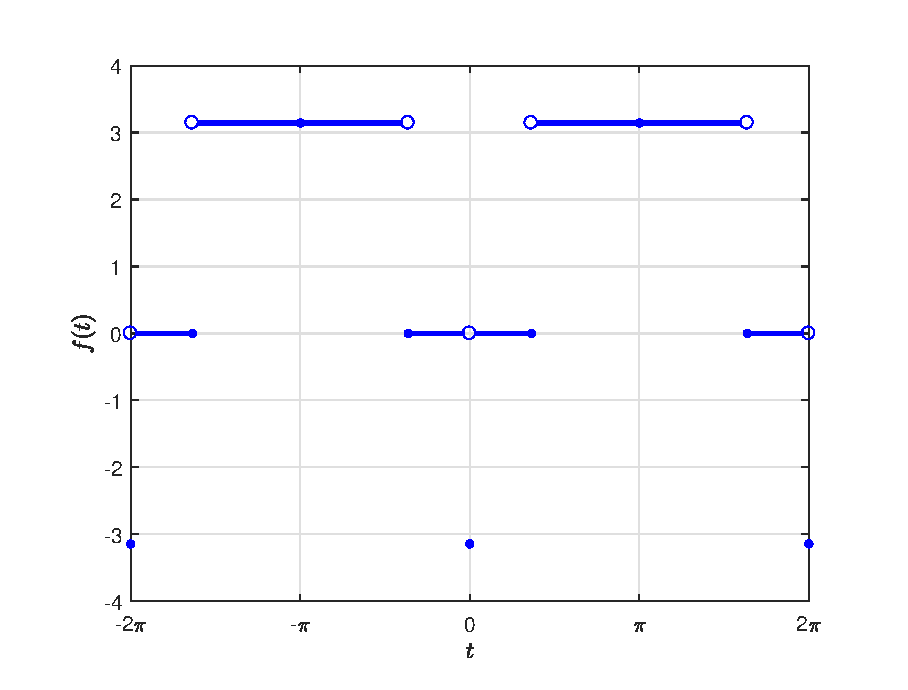
\includegraphics[width=\linewidth]{funk23.eps}
  \caption{$f(t)$ på intervallet $-2\pi \leq t \leq 2\pi$.}
  \label{fig:funk23}
\end{figure} 
\begin{figure}[h!]
  \centering
  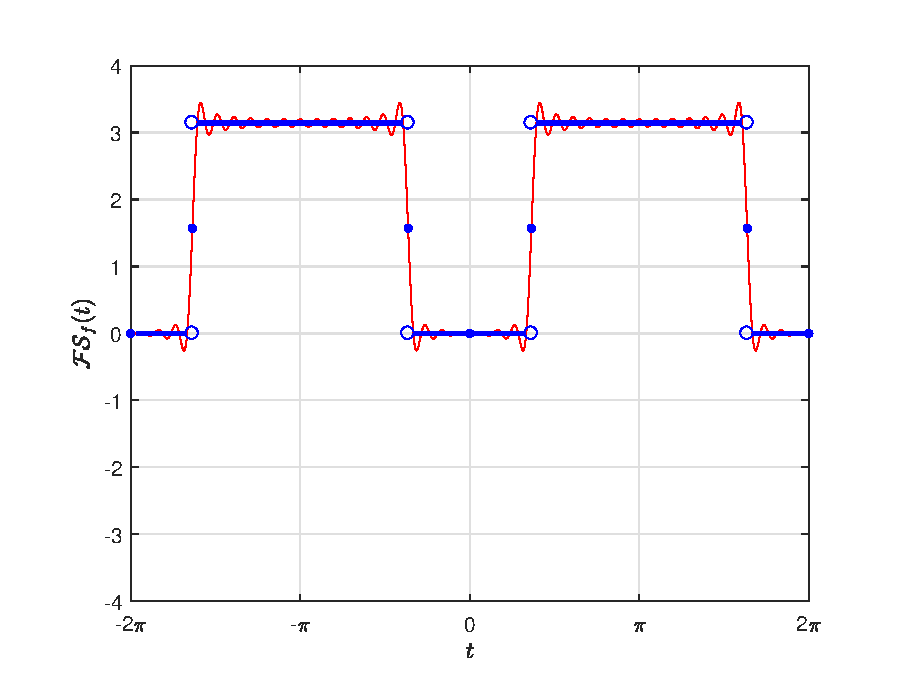
\includegraphics[width=\linewidth]{fourier23.eps}
  \caption{Gränsfunktionen till $\mathcal{FS}_f^{\text{trig}}(t)$ samt
    Fouriersumman för $20$ termer $S_{20}(t)$.}
  \label{fig:fourier23}
\end{figure} 

\FloatBarrier

\subsection*{c)}

För att bestämma summan $\sum_{k=1}^{+\infty}\frac{\sin(2k)}{k}$ utnyttjas
Fourierserien för $f(t)$ vid tidpunkten $t = \pi$.

\begin{align*}
  &\pi = 2 + 2\sum_{k=1}^{+\infty}(-1)^k\frac{\sin(2k)}{k}\cos(\pi k)\\
  &\iff \frac{\pi}{2} - 1 = \sum_{k=1}^{+\infty}(-1)^k\frac{\sin(2k)}{k}(-1)^k\\
  &\iff \sum_{k=1}^{+\infty}\frac{\sin(2k)}{k} = \frac{\pi}{2} - 1.
\end{align*}

\noindent Därefter ska summan $\sum_{k=1}^{+\infty}\frac{\sin^2(2k)}{k^2}$ beräknas. Här används Parsevals formel för trigonometriska Fourierserien

\begin{align*}
  \frac{1}{T}\int_{\text{p}}\left| f(t) \right|^2 dt = |c_0|^2 + \frac{1}{2} \sum_{k=1}^{+\infty} \left( |a_k|^2 + |b_k|^2\right).
\end{align*}

\noindent med $a_k = 2(-1)^k\frac{\sin(2k)}{k}$ och $b_k = 0$ fås då

\begin{align*}
  4 + \frac{1}{2}\sum_{k=1}^{+\infty}4\left| (-1)^k\right|^2\left|\frac{\sin(2k)}{k}\right|^2 &= \frac{1}{2\pi}\int_0^{2\pi}|f(t)|^2dt\\
  \iff 4 + 2\sum_{k=1}^{+\infty}\frac{\sin^2(2k)}{k^2} &= \frac{1}{2\pi}\int_{\pi-2}^{\pi+2}|\pi|^2dt = \frac{1}{2\pi}\left[\pi^2t\right]_{\pi-2}^{\pi+2}\\
  &=\frac{1}{2\pi}\left(\pi^3 + 2\pi^2 - \pi^3 + 2\pi^2\right) = 2\pi,
\end{align*}

\noindent vilket efter lite omskrivning ger

\begin{align*}
  \sum_{k=1}^{+\infty}\frac{\sin^2(2k)}{k^2} = \pi - 2
\end{align*}

\subsection*{d)}

Varken funktionen $f(t)$ eller gränsfunktionen till $\mathcal{FS}_f^{\text{trig}}(t)$ är kontinuerliga på intervallet $0 < t < 2\pi$, vilket orsakas av diskontinuiteten i $t = \pi - 2$ samt $t = \pi + 2$. Däremot är Fouriersumman för $n$-st termer $S_n(t)$ kontinuerlig då den är uppbyggd av kontinuerliga funktioner.

\subsection*{e)}

Fourierserien konvergerar inte likformigt mot sin gränsfunktion på intervallet
$0 < t < 2\pi$. Detta beror dels på gibs fenom, men även på diskontinuiteterna i
gränsfunktionen, vilket medför att supremumnormen alltid är större eller lika
med $\pi/2$, och serien kan därmed inte konvergera likformigt.

\section*{2.4}

Enligt uppgiften definieras dilogaritmen som

\begin{align*}
  \text{Li}_2 = \sum_{k=1}^{+\infty}\frac{z^k}{k^2}.
\end{align*}

\subsection*{a)}

För vilka värden konvergerar dilogaritmen?

Kvotestet ger här

\begin{align*}
  \kappa = \lim_{k\to\infty}\frac{\left|\frac{z^{k+1}}{(k+1)^2}\right|}{\left|\frac{z^k}{k^2}\right|} = \lim_{k\to\infty}\left| \frac{z^{k+1}k^2}{z^k(k+1)^2}\right| = |z|\lim_{k\to\infty}\frac{k^2}{(k+1)^2} = |z|.
\end{align*}

\noindent Dilogaritmen konvergerar för alla $z$ som uppfyller $\kappa < 1$, d.v.s. då $|z|
< 1$. Alltså för alla $z$ som innesluts av enhetscirkeln.

\subsection*{b)}

\begin{align*}
  \text{Li}\left(\frac{1}{2}\right)_2 \approx \sum_{k=1}^4\frac{(1/2)^k}{k^2} \approx 0.5802951.
\end{align*}

\noindent En uppskattning av detta fel fås genom att först approximera serien

\begin{align*}
	\sum_{k=1}^{+\infty}\frac{(1/2)^k}{k^2} &= \frac 12 + \frac{1}{2^2\cdot2^2} + \frac{1}{2^3\cdot3^2} + \ldots\\
										 &= \frac 12 \left( 1 + \frac{1}{2\cdot2^2} + \frac{1}{2^2\cdot3^2} + \ldots \right)\\
			  &\leq \frac 12 \sum_{k=0}^{+\infty}\frac{1}{8^k} = \frac 12 \cdot \frac{1}{1 - 1/8} = \frac 47,
\end{align*}

\noindent felupskattningen blir då

\begin{align*}
	\left| \frac 47 - 0.5802951 \right| = 0.008866529
\end{align*}

\subsection*{c)}

Om

\begin{align*}
  \text{Li}_2 \approx \sum_{k=1}^{N}\frac{1}{k^2}
\end{align*}

\noindent ska ha ett lika litet fel som i föregående uppgiften, d.v.s. ett fel på $0.008866529$ så tas $N$ fram med hjälp av resttermen för serien

\begin{align*}
  r_N = \sum_{N+1}^{+\infty}\frac{1}{k^2} \leq 0.008866529
\end{align*}

\noindent För att approximera $r_N$ görs en integraluppskattning

\begin{align*}
  r_N &= \sum_{N+1}^{+\infty}\frac{1}{k^2} \leq \int_N^{+\infty}\frac{1}{x^2}dx = \left[-\frac{1}{x}\right]_N^{+\infty}\\
  &= \left(-0 + \frac{1}{N}\right) \leq 0.0025 \implies N \geq 113.
\end{align*}

\noindent Det krävs alltså minst 113 termer för att få ett fel på 0.008866529.

\subsection*{d)}

Maple används för att dubbelkolla resultatet från föregående två deluppgifter.

För att beräkna felet i deluppg. b) görs följande räkningar

\begin{figure}[h!]
	\centering
	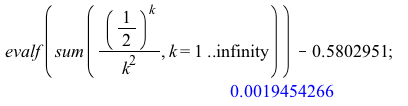
\includegraphics[width=0.5\linewidth]{maple_241.png}
	\caption{Mapleräkningar för feluppskattning i deluppgift b).}
	\label{fig:maple_241}
\end{figure}

\noindent Från Figur \ref{fig:maple_241} syns det fel som beräknades för hand är större än det egentliga felet som beräknades av Maple, vilket är förväntat om approximationen av serien är någorlunda bra.
För deluppgift c) stämmer resultatet som räknades för hand överens med det som Maple gav (se Figur \ref{fig:maple_242}).

\begin{figure}[h!]
	\centering
	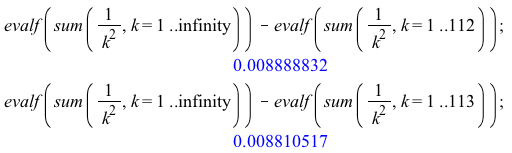
\includegraphics[width=0.63\linewidth]{maple_242.png}
	\caption{Kontrollräkning i Maple för resultatet från deluppgift c).}
	\label{fig:maple_242}
\end{figure}

\noindent Gränsen för att felet skall ligga under 0.008866529 går precis vid 113 termer, vilket Maple bekräftar.

\newpage
\appendix
\section{Maplekörningar för 2.1}\label{ap:maple}
\begin{figure}[h!]
	\centering
	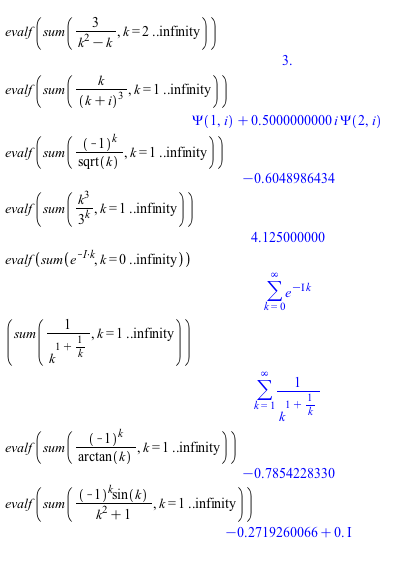
\includegraphics[width=\linewidth]{maple_1.png}
\end{figure}

\end{document}
